\documentclass[10pt,a4paper]{article}
\usepackage{amsmath}
\usepackage{amssymb}
\usepackage{graphicx}
\usepackage{color}
\usepackage{fancyhdr}
\usepackage{fancyvrb}
\usepackage[margin=3.5cm]{geometry}
\usepackage{framed}
\usepackage{enumerate}
\usepackage{textcomp}
\def\ket#1{\left|#1\right\rangle}
\def\bra#1{\left\langle#1\right|}
\def\braket#1{\left\langle#1\right\rangle}

\definecolor{linkcol}{rgb}{0.0, 0.0, 0.7}
\usepackage[colorlinks=true,urlcolor=linkcol,citecolor=black,linkcolor=linkcol]{hyperref}

\renewcommand{\theequation}{6.\arabic{equation}}
\setcounter{section}{6}
\renewcommand\thesection{\arabic{section}}
\renewcommand\thesubsection{\thesection.\arabic{subsection}}

\fancyhf{}
\lhead{\tiny Y.~D.~Chong (2021)}
\rhead{\scriptsize MH2801: Complex Methods for the Sciences}
\lfoot{}
\rfoot{\thepage}
\pagestyle{fancy}

\begin{document}
\setcounter{page}{40}

\noindent
{\Large \textbf{6. Complex Waves}}
\vskip 0.2in
\label{complex-waves}

Complex numbers are commonly used in the study of waves, such as
electromagnetic (light) waves, sound waves, and water waves.

\subsection{The wave equation}
\label{the-wave-equation}

A wave can be described by a function $f(x,t)$, called a
\textbf{wavefunction}, which specifies the value of some physical
quantity at each position $x$ and time $t$.

For simplicity, let us focus on the case of one spatial dimension, for
which $x$ is a single real number. We will also assume that the value
of the wavefunction is a number, rather than a more complicated object
such as a vector. For instance, a sound wave can be described by a
wavefunction whose value $f(x,t)$ is the local air pressure at
position $x$ and time $t$.

The wavefunction obeys a partial differential equation (PDE) called
the \textbf{time-dependent wave equation}:
\begin{align}
  \frac{\partial^2 f}{\partial x^2} = \frac{1}{v^2} \frac{\partial^2 f}{\partial t^2}, \;\;\; v \in\mathbb{R}^+.
\end{align}
The parameter $v$, which we take to be a positive real constant, is
called the \textbf{wave speed}, for reasons that will shortly become
clear.

Sometimes, we write the wave equation in the following form:
\begin{align}
  \left(\frac{\partial^2}{\partial x^2} - \frac{1}{v^2} \frac{\partial^2}{\partial t^2}\right) \; f(x,t) = 0.
\end{align}
This consists of a linear differential operator acting on $f(x,t)$,
which emphasizes that the wave equation is a linear PDE. Hence, any
linear superposition of solutions is also a solution.

\subsection{Real solutions to the wave equation}
\label{real-solutions-to-the-wave-equation}

We first consider real solutions to the wave equation. One family of
solutions are \textbf{travelling waves} of the form
\begin{align}
  f(x,t) = f_0 \, \cos\!\big(kx - \omega t + \phi\big),\quad\mathrm{where}\;\, \left|\frac{\omega}{k}\right| = v.
\end{align}
By direct substitution, we can verify that this satisfies the PDE.  We
call $f_0$ the \textbf{amplitude} of the wave, $\phi$ the
\textbf{phase}, $\omega$ the (angular) \textbf{frequency}, and $k$ the
\textbf{wavenumber}. By convention, $\omega$ is taken to be a positive
real number. However, $k$ can be either positive or negative, and its
sign determines the direction of propagation of the wave; the
magnitude of the wavenumber is inversely related to the wavelength
$\lambda$ by $\lambda = 2\pi/|k|$.

As $t$ increases, the wave moves to the right if $k$ is positive, or
to the left if $k$ is negative.  Here's one way to reason out why this
is the case. Consider introducing a small change in time, $\delta t$,
into the function $\cos(kx - \omega t + \phi)$. If, together with this
time shift, we change $x$ by $\delta x = (\omega/k)\, \delta t$, then
the change in the $kx$ term and the change in the $\omega t$ term
cancel, leaving the value of the cosine unchanged:

\begin{figure}[ht]
  \centering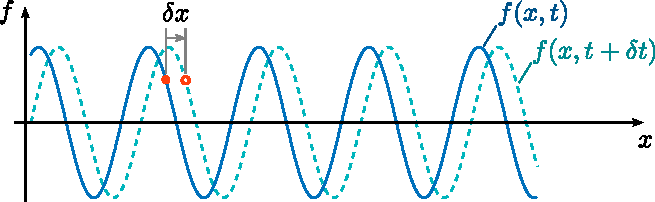
\includegraphics[width=0.6\textwidth]{wave_velocity}
\end{figure}

This implies that the wave shifts by $\delta x = (\omega/k)\, \delta
t$ during the time interval $\delta t$. Hence, the wave velocity is
\begin{align}
  \frac{\delta x}{\delta t} = \frac{(\omega/k)\,\delta t}{\delta t} = \frac{\omega}{k}.
\end{align}
As previously noted, $\omega$ is conventionally taken to be a positive
real number. Hence, positive $k$ implies that the wave is right-moving
(positive velocity), and negative $k$ implies the wave is left-moving
(negative velocity). Moreover, $v$ is the wave speed (i.e., the
absolute value of the velocity):
\begin{align}
  \left|\frac{\delta x}{\delta t}\right| = \frac{\omega}{\left|k\right|} = v.
\end{align}

\subsubsection{Standing waves}
\label{standing-waves}

Suppose we have two travelling wave solutions, with equal amplitude
and frequency, moving in opposite directions:
\begin{align}
  f(x,t) = f_0 \, \cos(kx - \omega t + \phi_1) + f_0 \cos(-kx - \omega t + \phi_2).
\end{align}
Here, we denote $k = \omega/c$.  Such a superposition is also a
solution to the wave equation, called a \textbf{standing wave}. It can
be re-written in a variable-separated form (i.e., as the product of a
function of $x$ and a function of $t$):
\begin{align}
  f(x,t) = 2f_0 \, \cos\big[kx + (\phi_1-\phi_2)/2\big]\, \cos\big[\omega t - (\phi_1+\phi_2)/2\big].
  \label{eq:standing}
\end{align}
This can be proven using the trigonometric addition formulas, but the
proof is tedious.

\subsection{Complex solutions to the wave equation}
\label{complex-solutions-to-the-wave-equation}

It is much easier to deal with the wave equation if we promote it into
a complex PDE by allowing $f(x,t)$ to be complex. The coordinate
variables $x$ and $t$ will remain real. We will also take the wave
speed $v$ to be real, for now.

From any complex solution to the wave equation, we can take the real
part to get a solution to the real PDE, thanks to linearity:
\begin{align}
  \left(\frac{\partial^2}{\partial x^2} - \frac{1}{v^2} \frac{\partial^2}{\partial t^2}\right) \mathrm{Re}\left[f(x,t)\right] = \mathrm{Re} \left[ \left(\frac{\partial^2}{\partial x^2} - \frac{1}{v^2} \frac{\partial^2}{\partial t^2}\right) f(x,t)\right] = 0.
\end{align}
There exists a nice set of complex solutions to the wave equation,
called \textbf{complex travelling waves}, which take the form
\begin{align}
  f(x,t) = A \, e^{i(kx - \omega t)} \quad\mathrm{where}\;\; \left|\frac{\omega}{k}\right| = v.
\end{align}
This can be shown to satisfy the PDE via direct substitution.  The
complex constant $A$ is called the \textbf{complex amplitude} of the
wave. Consider what happens if we take the real part of the above
solution:
\begin{align}
  \mathrm{Re}\Big[A \, e^{i(kx - \omega t)}\Big] &= \mathrm{Re}\Big[ |A|\, e^{i\mathrm{arg}[A]} \; e^{i(kx - \omega t)}\Big] \\
  &= |A|\; \mathrm{Re}\Big[ e^{i\mathrm{arg}[A]} \, e^{i(kx - \omega t)}\Big] \\
  &= |A|\; \cos\!\big(kx - \omega t + \mathrm{arg}[A]\big)
\end{align}

Comparing this to the real solution from
Section~\ref{real-solutions-to-the-wave-equation}, we see that $|A|$
serves as the amplitude of the real wave, while $\mathrm{arg}(A)$
serves as the phase factor $\phi$. The complex solution is thus more
succinct than the real solution: a single complex parameter $A$
combines the roles of two parameters in the real solution.

The complex representation also makes wave superpositions easier to
handle. As an example, consider the superposition of two
counter-propagating waves of equal amplitude and frequency, with
arbitrary phases. Using complex travelling waves, we can calculate the
superposition with a few lines of algebra:
\begin{align}
  f(x,t) &= |A| \, e^{i(kx - \omega t + \phi_1)} + |A| \, e^{i(-kx - \omega t + \phi_2)} \\
  &=  |A|\, \left(e^{i(kx + \phi_1)} + e^{-i(kx - \phi_2)}\right)\, e^{-i\omega t} \\
  &= |A|\, \left(e^{i[kx + (\phi_1-\phi_2)/2]} + e^{-i[kx + (\phi_1 - \phi_2)/2]}\right)\, e^{i(\phi_1 + \phi_2)/2} \,e^{-i\omega t} \\
  &= \displaystyle 2\,|A|\, \cos\left[kx + (\phi_1-\phi_2)/2\right] \,e^{-i[\omega t -(\phi_1+\phi_2)/2]}.
\end{align}
Taking the real part yields our previous result \eqref{eq:standing},
without the need for tedious manipulations of trigonometric formulas.

\subsection{Waves in 3D space}
\label{waves-in-3d-space}

The wave equation can be generalized to three spatial dimensions by
replacing $f(x,t)$ with a wavefunction that depends on three spatial
coordinates, $f(x,y,z,t)$.  The second-order derivative in $x$ is then
replaced by second-order derivatives in each spatial direction:
\begin{align}
  \left(\frac{\partial^2}{\partial x^2} + \frac{\partial^2}{\partial y^2} + \frac{\partial^2}{\partial z^2} - \frac{1}{v^2} \frac{\partial^2}{\partial t^2}\right) \; f(x,y,z,t) = 0.
  \label{eq:3dwave}
\end{align}
This PDE supports complex plane wave solutions of the form
\begin{align}
  f(x,y,z,t) = A \, \exp\left[i\left(\vec{k} \cdot \vec{r} - \omega t\right)\right],
\end{align}
where
\begin{align}
  \vec{k} = \begin{bmatrix}k_x\\k_y\\k_z\end{bmatrix}, \;\;\; \vec{r} = \begin{bmatrix}x\\y\\z\end{bmatrix}, \;\;\;\frac{\omega}{\sqrt{k_x^2 + k_y^2 + k_z^2}} = v.
\end{align}
Again, we can verify that this is a solution by direct substitution.
The \textbf{wave-vector} $\vec{k}$ is a generalization of our previous
one-dimensional $k$; it points in the direction in which the wave
travels.

\subsection{Harmonic waves}
\label{harmonic-waves}
We are often interested in waves undergoing \textbf{harmonic
  oscillation}, i.e.~varying sinusoidally with a constant frequency
$\omega$ everywhere in space.  Such waves can be described by
wavefunctions of the form
\begin{align}
  f(x,y,z,t) = \psi(x,y,z) \, e^{-i\omega t}.
\end{align}
By writing the wavefunction in this form, we are performing a
separation of variables between $\vec{r}$ and $t$. This is a common
strategy for solving linear PDEs: assuming we can find harmonic
solutions for each frequency $\omega$, they can be linearly combined
to construct more general solutions.

By direct substitution into the 3D wave equation \eqref{eq:3dwave}, we
can show that $\psi(x)$ obeys
\begin{align}
  \left[\frac{\partial^2}{\partial x^2} + \frac{\partial^2}{\partial y^2} + \frac{\partial^2}{\partial z^2} + \left(\frac{\omega}{v}\right)^2\right] \, \psi(x,y,z) = 0.
\end{align}
This is called the \textbf{time-independent wave equation}, and is
related to the time-dependent wave equation by the replacement
$\partial/\partial t \rightarrow -i\omega$.

\subsubsection{Waves in complex media}
\label{waves-in-complex-media}

So far, our discussion has been limited to waves propagating in a
uniform, energy-conserving medium with a fixed wave speed $v$. There
are two important generalizations of this scenario: (i) non-uniform
media, in which the wave speed varies with position, and (ii) energy
non-conserving media, in which the waves lose or gain energy as they
propagate. To describe such phenomena, we define
\begin{align}
  v = \frac{c}{n},
\end{align}
where $n$ is called the \textbf{refractive index}, and the constant
$c$ is the wave speed in the limit $n = 1$.  In the case of
electromagnetic waves, $c$ is the speed of light in a vacuum.

If the refractive index is now allowed to vary with position, the wave
equation in the harmonic representation becomes
\begin{align}
  \left[\frac{\partial^2}{\partial x^2} + \frac{\partial^2}{\partial y^2} + \frac{\partial^2}{\partial z^2} + n^2(x,y,z)\, \left(\frac{\omega}{c}\right)^2\right] \, \psi(x,y,z) = 0.
\end{align}

\subsubsection{Wave amplification and attenuation}
\label{gainloss}

By allowing the refractive index $n$ to be complex, the wave equation
can describe the phenomena of \textbf{wave amplification} (which is
also called \textbf{gain}) and \textbf{wave attenuation} (also called
\textbf{loss}). Wave amplification and attenuation occur in many
different physical contexts; for example, the amplification of light
waves is the underlying basis for the laser.

To study the implications of complex $n$, let us go back to
one-dimensional space and the simple scenario of a
position-independent refractive index. The time-independent wave
equation reduces to
\begin{align}
  \left[\frac{d^2}{d x^2} + n^2\, \left(\frac{\omega}{c}\right)^2\right] \, \psi(x) = 0.
\end{align}
We now let $n$ be complex, while keeping $\omega$ and $c$ as positive
real numbers. The solutions to the ODE have the form
\begin{align}
  \psi(x) = A \exp\left(\pm \frac{in\omega}{c}x\right),\;\;\;\mathrm{where}\;\; A \in \mathbb{C}.
  \label{eq:gainloss-wave}
\end{align}
Let us write the complex refractive index as
\begin{align}
  n = n' + i n'',\quad \textrm{where}\;\, n',n'' \in \mathbb{R}.
\end{align}
Then
\begin{align}
  \psi(x) = A \exp\left[\pm in'(\omega/c)x\right]\, \exp\left[\mp n''(\omega/c)x\right].
\end{align}
The first exponential factor describes the oscillation of the
wavefunction, with the $\pm$ sign determining whether the harmonic
wave is moving to the right or to the left. The second exponential
describes the amplification or attenuation of the wave.  If $n'' \ne
0$, the amplitude varies exponentially with $x$. Thus, depending on
the signs of the various parameters, the wave might grow exponentially
along its direction of propagation, which corresponds to
amplification, or decrease exponentially along its direction of
propagation, which corresponds to damping.

\subsubsection{Wave refraction (optional topic)}

The time-independent wave equation can be used to study the refraction
of waves passing between different media.  Consider, as shown in the
figure, two semi-infinite media with refractive indices $n_1$ (for $y
> 0$) and $n_2$ (for $y < 0$).  We assume that $n_1$ and $n_2$ are
positive real numbers, and consider waves propagating in the $x$-$y$
plane, ignoring the $z$ direction.

\begin{figure}[h]
  \centering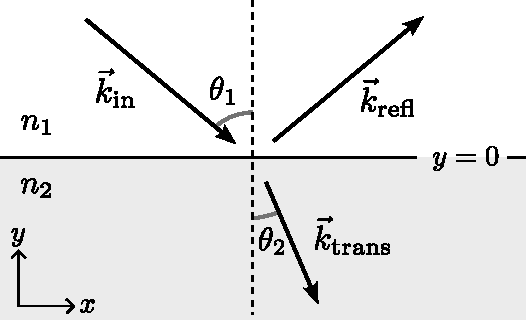
\includegraphics[width=0.4\textwidth]{refraction}
\end{figure}

Let us look for a wavefunction of the form
\begin{equation}
  \psi(x,y) = e^{ikx} \, \Phi(y).
  \label{psisep}
\end{equation}
(Why do we seek such a solution?  Because the system is
translationally symmetric along $x$, so it ought to support elementary
solutions with a simple wave-like variation in $x$.  This is an
example of the physics principle known as Noether's Theorem.)

Substituting Eq.~\eqref{psisep} into the time-independent wave
equation reduces it to
\begin{equation}
  \left[\frac{d^2}{dy^2} - k^2 + \frac{n(y)^2 \omega^2}{c^2} \right]
  \Phi(y) = 0.
  \label{wave1dode}
\end{equation}
In the upper medium ($y > 0$), where $n = n_1$, there are solutions
$\exp(\pm i\kappa_1 y)$ where
\begin{equation}
  k^2 + \kappa_1^2 = \frac{n_1^2 \omega^2}{c^2}.
  \label{kk}
\end{equation}
Suppose $k < n_1 \omega / c$, so that $\kappa_1$ is real.  We let
$\Phi(y)$ be a superposition of the two solutions:
\begin{equation}
  \Phi(y) = e^{-i\kappa_1 y} + r e^{i\kappa_1 y}, \;\;\; \mathrm{where}\;\;
  r \in \mathbb{C}.
\end{equation}
Putting the $x$-dependence back in, we get
\begin{equation}
  \psi(x,y) = e^{i\vec{k}_{\mathrm{in}}\cdot r}
  + r e^{i\vec{k}_{\textrm{refl}}\cdot r}, \quad(\textrm{for} \; y > 0),
  \label{psiinr}
\end{equation}
where
\begin{equation}
  \vec{k}_{\textrm{in}} = \begin{bmatrix}k \\ -\kappa_1 \end{bmatrix}, \;\;\;
  \vec{k}_{\textrm{refl}} = \begin{bmatrix}k \\ \kappa_1 \end{bmatrix}.
\end{equation}
Eq.~\eqref{psiinr} describes a superposition of an \textbf{incident
  wave} and a \textbf{reflected wave}, with wave-vectors
$\vec{k}_{\textrm{in}}$ and $\vec{k}_{\textrm{refl}}$ respectively.
The complex \textbf{reflection coefficient} $r$ describes the
reflected wave's amplitude and phase relative to the incident wave.
Note that $\vec{k}_{\textrm{in}}$ and $\vec{k}_{\textrm{refl}}$ have
the same $x$-component ($k$) and exactly opposite $y$-components ($\pm
\kappa_1$); this is consistent with the \textbf{law of reflection},
which states that the angle of reflection matches the angle of
incidence.  The angle of incidence $\theta_1$ is
\begin{equation}
  \sin(\theta_1) = \frac{k}{\sqrt{k^2+\kappa_1^2}} = \frac{ck}{n_1\omega}.
  \label{sintheta1}
\end{equation}

Part of the incident wave may also be transmitted into the lower
medium ($y < 0$).  Returning to Eq.~\eqref{wave1dode}, let $\Phi(y) =
t \exp(-i\kappa_2y)$, so that the transmitted wavefunction is
\begin{equation}
  \psi(x,y) = t e^{i\vec{k}_{\mathrm{trans}}\cdot \vec{r}}, \quad(\textrm{for} \; y < 0),
  \label{psilower}
\end{equation}
where $t$ is called the \textbf{transmission coefficient}, and
\begin{equation}
  \vec{k}_{\mathrm{trans}} =
  \begin{bmatrix}k \\ -\kappa_2 \end{bmatrix}, \quad
  k^2 + \kappa_2^2 = \frac{n_2^2\omega^2}{c^2}.
  \label{psilower2}
\end{equation}
Note that Eq.~\eqref{psilower} does not include a wave traveling in
the $+y$ direction, on physical grounds: we are interested in the
situation where a wave is incident from the upper medium and there is
no wave incident from the bottom.  Now, if $k < n_2 \omega / c$,
then $\kappa_2$ is real, and we can define the angle of transmission
$\theta_2$ by
\begin{equation}
  \sin(\theta_2) = \frac{k}{\sqrt{k^2 + \kappa_2^2}} =
  \frac{ck}{n_2\omega}.
  \label{sintheta2}
\end{equation}
Combining Eq.~\eqref{sintheta1} and \eqref{sintheta2} gives
\begin{equation}
  \frac{\sin(\theta_1)}{\sin(\theta_2)} = \frac{n_2}{n_1}.
\end{equation}
We have thus derived \textbf{Snell's law}, also known as the
\textbf{law of refraction}.

\subsubsection{Evanescent waves (optional topic)}

In the above study of wave refraction, we assumed that in the $x$
direction, along the interface, the wavenumber $k$ satisfies
\begin{equation*}
  k < \frac{n_1\omega}{c} \;\;\textrm{and}\;\;
  k < \frac{n_2\omega}{c}.
\end{equation*}
These conditions allow $\kappa_1$ and $\kappa_2$ (i.e., the
wavenumbers along $y$ in each medium) to be real.  But what if one of
the conditions is violated?  Suppose that
\begin{equation}
  \frac{n_2\omega}{c} < k < \frac{n_1\omega}{c}.
  \label{evanescent_condition}
\end{equation}
Then $\kappa_1$ remains real, but $\kappa_2 =
\sqrt{(n_2\omega/c)^2-k^2}$ becomes imaginary.  Note that this implies
$n_2 < n_1$ (i.e., the wave is incident from the medium with the
\textit{higher} refractive index). Using Eq.~\eqref{sintheta1}, let
write $k$ in terms of the angle of incidence,
\begin{equation}
  k = \frac{n_1 \omega \sin(\theta_1)}{c}.
\end{equation}
Plugging this into Eq.~\eqref{evanescent_condition} yields
\begin{align}
  \frac{n_2\omega}{c} &< \frac{n_1 \omega \sin(\theta_1)}{c} \\
  \Leftrightarrow \qquad
  \theta_1 &> \theta_c \equiv  \sin^{-1}\left[\frac{n_2}{n_1}\right].
\end{align}
Thus, when the angle of incidence exceeds the \textbf{critical angle}
$\theta_c$, there is no plane wave transmitted into the lower-index
medium.

In that case, what happens to the wavefunction in the lower-index
medium?  Let us take $\kappa_2 = i \gamma_2$ where $\gamma_2 \in
\mathbb{R}^+$.  Plugging this into the $y < 0$ solution,
Eqs.~\eqref{psilower}--\eqref{psilower}, gives
\begin{equation}
  \psi(x,y) = t e^{ikx} \, e^{\gamma_2 y},
\end{equation}
where
\begin{align}
  \gamma_2 &= \sqrt{k^2 - \frac{n_2^2\omega^2}{c^2}} \\
  &= \sqrt{\left[n_1\sin(\theta_1)\right]^2 - n_2^2} \;\cdot\,\frac{\omega}{c}.
\end{align}
This is called an \textbf{evanescent wave}.  In the $x$ direction
(parallel to the interface) it behaves like an traveling wave, but in
the $y$ direction it decays exponentially away from the interface.
Evanescent waves have numerous applications in optics and other areas.
For example, they underpin the technique called
\href{https://en.wikipedia.org/wiki/Total_internal_reflection_fluorescence_microscope}{Total
  Internal Reflection Fluorescence (TIRF) microscopy}, which is used
to make extremely high-resolution images of biological cells.

\subsection{Exercises}
\label{exercises}

\begin{enumerate}
\item
  Consider the 1D wave equation in a enclosed box of length $L$ and
  uniform refractive index $n\in\mathbb{R}$. The walls of the box are
  at $x = -L/2$ and $x = L/2$, and the wavefunction goes to zero at
  these points: $\psi(\pm L/2) = 0$ (i.e., Dirichlet boundary
  conditions). Show that $\psi(x) = 0$ for all $x$, \emph{except}
  for certain discrete values of the frequency $\omega$. Find these
  frequencies, and the corresponding non-zero solutions $\psi(x)$.

\item
  As discussed in Section~\ref{gainloss}, a harmonic travelling wave
  in an energy-nonconserving medium is described by
  \begin{equation}
    \left[\frac{d^2}{d x^2} + n^2\, \left(\frac{\omega}{c}\right)^2\right] \, \psi(x) = 0,
  \end{equation}
  where $n$ is a complex number. (As usual, $\omega$ and $c$ are
  assumed to be positive real numbers.) Show that the relative sign of
  $\mathrm{Re}(n)$ and $\mathrm{Im}(n)$ determines whether the wave
  experiences amplification or dissipation, and that the result does
  not depend of the wave's propagation direction.
  \hfill{\scriptsize [solution~available]}

\item
  When the refractive index is complex, can the real part of the
  complex wavefunction be regarded as the solution to the same wave
  equation? If not, derive a real differential equation whose solution
  is the real part of Eq.~\eqref{eq:gainloss-wave}.
\end{enumerate}

    
\end{document}
